\documentclass[journal]{IEEEtran}
\IEEEoverridecommandlockouts
%%%%%%%%%%%%%%%%%%%%%%%%%%%%%%%%%%%%%%
%%%%%%%% PRINCIPALES PAQUETES %%%%%%%%
%%%%%%%%%%%%%%%%%%%%%%%%%%%%%%%%%%%%%%
\usepackage{fancyhdr}
\usepackage{graphicx}
\usepackage[spanish, es-tabla]{babel}
\usepackage[utf8]{inputenc}
\usepackage{color}
\usepackage{hyperref}
\usepackage{wrapfig}
\usepackage{array}
\usepackage{multirow}
\usepackage{adjustbox}
\usepackage{nccmath}
%\usepackage{anysize}
\usepackage{subfigure}
\usepackage{amsfonts,latexsym} % para tener disponibilidad de diversos simbolos
\usepackage{enumerate}
\usepackage{booktabs}
\usepackage{float}
\usepackage{threeparttable}
\usepackage{array,colortbl}
\usepackage{ifpdf}
\usepackage{rotating}
\usepackage{cite}
\usepackage{stfloats}
\usepackage{url}
\usepackage{listings}
\usepackage{tikz}
\usepackage{hyperref}
\usepackage{multicol}

\definecolor{gray97}{gray}{.97}
%Estilo del código
\lstset{ frame=Ltb,
	framerule=0pt,
	aboveskip=0.5cm,
	framextopmargin=3pt,
	framexbottommargin=3pt,
	framexleftmargin=0.4cm,
	framesep=0pt,
	rulesep=.4pt,
	backgroundcolor=\color{gray97},
	rulesepcolor=\color{black},
	%
	stringstyle=\ttfamily,
	showstringspaces = false,
	basicstyle=\ttfamily,
	commentstyle=\color{blue},
	keywordstyle=\color{red},
	%
	numbers=left,
	numbersep=15pt,
	numberstyle=\ttfamily,
	numberfirstline = false,
	breaklines=true,
}
%%%%%%%%%%%%%%%%%%%%%%%%%%%%%%%%%%%%%%%%%%%
%%% CREAR Y REESCRIBIR ALGUNOS COMANDOS %%%
%%%%%%%%%%%%%%%%%%%%%%%%%%%%%%%%%%%%%%%%%%%
\newcolumntype{P}[1]{>{\centering\arraybackslash}p{#1}}
%% Se crea un nuevo tipo de columna llamada P.
\newcommand{\tabitem}{~~\llap{\textbullet}~~}
\newcommand{\ctt}{\centering\scriptsize\textbf}
%%\ctt abrevia el comando \centering\scriptsize\textbf
\newcommand{\dtt}{\scriptsize\textbf} %%\dtt abrevia el comando \scriptsize\textbf
\renewcommand\IEEEkeywordsname{Palabras clave}

\renewcommand\IEEEkeywordsa{Key words}
\renewcommand\abstracteee{Abstract}

%%%%%%%%%%%%%%%%%%%%%%%%%%%%%%%%%%%%%%%%%%%

\graphicspath{ {Figs/} }  %%Ruta donde se encuentran las imágenes, que esté vacio indica que las imagenes están dentro de la misma carpeta que contiene el archivo .tex

%%%%%%%%%%%%%%%%%%%%%%%%%%%%%%%%%%%%%%%%%%%%%%%%%%%%%%%%%%
%%% ENCABEZADO DE LAS PÁGINAS  %%%%%%%%%%%%%%
%%%%%%%%%%%%%%%%%%%%%%%%%%%%%%%%%%%%%%%%%%%%%%%%%%%%%%%%%%
\newcommand{\MYhead}{\smash{\scriptsize
		\hfil\parbox[t][\height][t]{\textwidth}{\centering
			\begin{picture}(0,0)
				\put(-15,-20){
\includegraphics[width=4CM]{Figs/logo UV.png}} \end{picture}
			\hspace{6.4cm}
			PROYECTO - FÍSICA COMPUTACIONAL II-2022\hspace{5.15cm}
			\, \\
			\hspace{5.2cm} Prof. Karem Rodríguez\hspace{3cm} Enero
			2023\\
			\underline{\hspace{ \textwidth}}}\hfil\hbox{}}}
\makeatletter
% normal pages
\def\ps@headings{%
	\def\@oddhead{\MYhead}%
	\def\@evenhead{\MYhead}}%
% title page
\def\ps@IEEEtitlepagestyle{%
	\def\@oddhead{\MYhead}%
	\def\@evenhead{\MYhead}}%
\makeatother
% make changes take effect
\pagestyle{headings}
% adjust as needed
\addtolength{\footskip}{0\baselineskip}
\addtolength{\textheight}{-1\baselineskip}
%%%%%%%%%%%%%%%%%%%%%%%%%%%%%%%%%%%%%%%%%%%%%%%%%%%%%%%%%%
%%%%%%%%%%%%%%%%%%%%%%%%%%%%%%%%
%%%%% INICIO DEL DOCUMENTO %%%%%
%%%%%%%%%%%%%%%%%%%%%%%%%%%%%%%%
\begin{document}
%%%%%%%%%%%%%%%%%%%%%%%%%%%%
%%% TÍTULO DEL DOCUMENTO %%%
%%%%%%%%%%%%%%%%%%%%%%%%%%%%
\title{IV. PROPAGACIÓN DE ENFERMEDADES}
%%%%%%%%%%%%%%%%%%%%%%%%%%%%
%%%%%%%%% AUTORES %%%%%%%%%
%%%%%%%%%%%%%%%%%%%%%%%%%%%
\author{Andrés Felipe Valencia \\
	\textit{andres.valencia.fonseca@correounivalle.edu.co}\\% stops a space
	\and
	Nicolás Aguilera García \\
	\textit{nicolas.aguilera@correounivalle.edu.co}\\
	\thanks{El presente documento corresponde al articulo final del
		proyecto de Fisica computacional}} %\thanks anexa una nota a pie de página donde se puede colocar alguna información sobre la naturaleza del documento.
%%%%%%%%%%%%%%%%%%%%%%%%%%%

% Comando que indica la generación del título
\maketitle

%%%%%%%%%%%%%%%%%%%%%
%%%%%% RESUMEN %%%%%%
%%%%%%%%%%%%%%%%%%%%%
\begin{abstract}

\end{abstract}
% En el resumen no se recomienda colocar citaciones bibliográficas.

%%%%%%%%%%%%%%%%%%%%%%
%%% PALABRAS CLAVE %%%
%%%%%%%%%%%%%%%%%%%%%%
\begin{IEEEkeywords}

\end{IEEEkeywords}
%%%%%%%%%%%%%%%%%%%%%%
%\IEEEpeerreviewmaketitle

\begin{abstracteee}

\end{abstracteee}
% En el resumen no se recomienda colocar citaciones bibliográficas.

%%%%%%%%%%%%%%%%%%%%%%
%%% PALABRAS CLAVE %%%
%%%%%%%%%%%%%%%%%%%%%%
\begin{IEEEkeywordsa}

\end{IEEEkeywordsa}

%%%%%%%%%%%%%%%%%%%%%%%%%%%%%%%%%%%%%
%%% PRIMERA SECCIÓN DEL DOCUMENTO %%%
%%%%%%%%%%%%%%%%%%%%%%%%%%%%%%%%%%%%%
\section{Introducción}
\IEEEPARstart{E}{l} presente trabajo es el desarrollo numérico, bajo el uso de
lenguaje \textbf{\textit{C++}},
orientado al análisis matemático del modelo epidemiológico Ross \cite{Ross} y
McKendrick \cite{Kermack} a nivel poblacional conocido como modelo
\textbf{\textit{SIR}}.
Es a través de la modelación de procesos biológicos que la epidemiología
teórica recibe su mayor aporte.
Así que se opta por solucionar mediante el método de
\textbf{\textit{Runge-Kutta 4}} el conjunto de ecuaciones acopladas del modelo,
considerando de manera particular las condiciones
iniciales, y los parámetros propios de la enfermedad.

\subsection{Modelo de Kermack y McKendrick}

El estudio fundamental de Kermack \cite{Ross} y McKendrick \cite{Kermack} ha
sido de gran importancia en las últimas décadas. Su modelo
\textbf{\textit{SIR}}, susceptible-infeccioso-recuperado, y sus variaciones,
se han convertido en modelos básicos para sistemas no lineales que son
utilizados no solo por estudiantes interesados en aplicaciones matemáticas en
biología,
sino también para explicar a responsables de políticas, epidemiólogos y
expertos en salud pública la importancia del estudio de dinámica en
enfermedades contagiosas.\newline

Los campos de salud pública y epidemiología han sido dominados, con buenas
razones, por el uso de modelos estadísticos, sin embargo, se espera,
que el uso de modelos dinámicos aporte una nueva perspectiva, ya que permite a
teóricos y prácticos formular nuevas preguntas dentro de un marco que permite
explorar el impacto de intervenciones en la dinámica de transmisión de
enfermedades contagiosas.
Además, los modelos utilizados deben dar cuenta de los mecanismos responsables
de los patrones observados en la transmisión de una enfermedad contagiosa.
Este proceso ayuda a identificar, cuantificar, evaluar e implementar políticas
de intervención dirigidas a reducir el impacto de la epidemia o incluso brotes
pandémicos a través de la reducción del impacto de estos mecanismos.

\subsection{Modelos de Compartimentos}\label{Modelos}
%%%MOTROS ODELOS SI, SIR, SIS, Y SIRS VACUNACIÓN%%%%%%%%%%%
Los modelos compartimentales constituyen una técnica para simplificar la
modelización matemática que describe el flujo de material en sistemas
biológicos \cite{compartimientos}.
Estos modelos, se dividen en un número de compartimentos por los que circula el
material con flujos de entrada y salida. Este modelo
sirve para simular diferentes interacciones, entre ellas una de sus
aplicaciones se da en la epidemiología. Por lo general, un modelo
epidemiológico de compartimientos, se divide en clases y subclases de
individuos, y se estiman tasas de transición, para modelar el comportamiento
en base a un sistema de ecuaciones diferenciales.\\
\newline
En particular si la población se clasifica, en susceptibles $S$, infectados $I$
y recuperados $R$, se tienen los siguientes tipos de modelos;
\begin{enumerate}
	\item \textbf{\textit{SI}} la enfermedad del SIDA es un ejemplo que se
	      ajusta a este modelo \cite{SIDA}, aunque actualmente se está desarrollando
	      modelos mucho mas complejos para tratar esta enfermedad.
	\item \textbf{\textit{SIR}} Sirve para describir enfermedades virales,
	      como la rubéola o la sarampión \cite{Rubeola}.
	\item \textbf{\textit{SIS}} Modela el caso en que los individuos
	      infectados pueden retornar a la clase susceptible, es decir no adquieren
	      inmunidad. El dengue \cite{Dengue} es una enfermedad de este tipo.
	\item \textbf{\textit{SIRS}} Es un modelo con capacidad de soporte,
	      esto significa que el número de susceptibles no crece indefinidamente, puede
	      modelar la influenza \cite{Influenza}.
	\item \textbf{\textit{SIRS-V}} Recoge los modelos anteriores, y además
	      modela la capacidad de vacunación sobre la población \cite{Vacunacion}, siendo
	      este modelo uno de los mas completos.
\end{enumerate}

\begin{figure}[H]
	\centering
	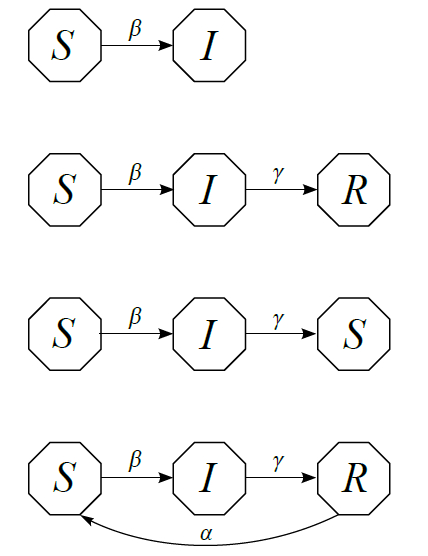
\includegraphics[scale=0.34]{Modelos.png}
	\caption{Modelos tipo SI, SIR, SIS y SIRS de compartimentos}
\end{figure}
%%%%%%%%%%%%%%%%%%%%%%%%%%%%%%%%%%%%%%
%%%MMODELO SIR%%%%%%%%%%%%%
\subsection{Modelo SIR}
Según este modelo \cite{Anderson} los individuos de la población
sobre la cual actúa la enfermedad, que en principio se considera constante, se
clasifican en los siguientes grupos:

\begin{itemize}
	\item \textbf{Susceptibles}, son aquellos individuos sanos pero que en
	      potencia se pueden
	      enfermar.
	\item \textbf{Infectados}, son los individuos enfermos.
	\item \textbf{Removidos}, son aquellos que se han recuperado, y
	      permanecen inmune a la misma sin poder propagarla.
\end{itemize}

Se denota por $S(t)$, $I(t)$ y $R(t)$ el número de individuos susceptibles,
infectados y removidos respectivamente.
En su versión más simple el modelo \textbf{\textit{SIR}} supone la siguiente
retroalimentación $S \rightarrow I \rightarrow R$.\newline

Si consideramos una relación mas simple, que nos da cuenta de la relación entre
cada población con la población total $N$, de este modo;
\begin{equation} \label{poblaciones}
	\begin{split}
		s(t) = \frac{S(t)}{N},\\
		i(t) = \frac{I(t)}{N},\\
		r(t) = \frac{R(t)}{N}\\
	\end{split}
\end{equation}

Para describir entonces la dinámica de la enfermedad se propone el siguiente
sistema:

\begin{equation}\label{SIR}
	\begin{split}
		\frac{ds}{dt} = -bs(t)i(t),\\
		\frac{di}{dt} = bs(t)i(t)-ki(t),\\
		\frac{dr}{dt} = -ki(t)\\
	\end{split}
\end{equation}

Donde $b$ y $k$, son parámetros de la enfermedad, más estrictamente; $k$ es la
tasa de remoción de individuos infectados, quiere decir, una
número de miembros infectados que pasa a la clase de removidos por unidad de
tiempo.\\
Mientras $b$ es la tasa de contacto, representa la capacidad de infectar que
posee la enfermedad. En el modelo que estamos considerando los parámetros
depende de la enfermedad
particular que se estudié, y por lo tanto, puede también depender de factores
sociales y
de comportamiento. En general es difícil estimar ambas constantes.

%%% SUPOSICIONES DEL MODELO%%%%
\subsubsection{Hipótesis}
Este modelo, se sustenta bajo ciertas suposiciones, que limitan la capacidad de
aplicación del mismo, lo que lo convierte en un modelo sencillo,
más sin embargo superar estas suposiciones involucra mejorar el modelo, en la
sección \ref{Modelos} se muestran algunos ejemplos. En el caso del modelo
\textbf{\textit{SIR}} \ref{SIR}
sobre el que se trabaja, se parte bajo los siguientes supuestos;

\begin{enumerate}
	\item  El tamaño de la población $N$ es constante, es decir no se
	      consideran muertes, ni se tiene en cuenta los nacimientos dentro de la
	      población
	      durante la epidemia, esto implica la relación;
	      \begin{equation}\label{suposicion}
		      \frac{d(s+i+r)}{dt} = 0
	      \end{equation}
	      Esta hipótesis se consigue de manera razonable en epidemias de
	      corta duración.
	\item La enfermedad únicamente se propaga, bajo la ley de acción de
	      masas entre la población de susceptibles e infectados, como
	      tambien se supone que la transmisión se rige por la incidencia
	      común, entre las mismas poblaciones, lo que se refleja en el parámetro
	      $b$, una taza constante de contagios que es proporcional al
	      numero de contactos entre los individuos susceptibles e infectados.
	\item La taza de recuperación de individuos infectados $k$, no varia
	      bajo la dinámica de las poblaciones ni de la enfermedad, es decir es una
	      constante.
\end{enumerate}

\section{Metodología}
%%%%ESTABLECER METOOD DE SOLUCIÓN, CONDICIONES INICIALES, Y PARAMETROS%%%%%%%%%%%%%%%
La matemática ha sido una herramienta que ha generado un gran avance dentro de
cada una de las
disciplinas de la biología moderna, acompañada de la estadística y la
computación. El propósito de este trabajo
es solucionar el problema de los modelos epidemiológicos, y simular el
comportamiento de las poblaciones, bajo
circunstancias establecidas, para llevarlo a cabo, se busca implementar
computacionalmente métodos de soluciones numéricas.\\

El conjunto de ecuaciones diferenciales acopladas \ref{SIR}, se convierte un
problema de alto nivel analítico,
no obstante existen desarrollos que tratan las soluciones de ese tipo de
modelos, dando soluciones algebraicas \cite{Sulucion_analitica}.
Sin embargo el desarrollo de la computación ha permitido implementar de manera
mas eficiente técnicas o métodos
para solucionar numéricamente ecuaciones diferenciales, en particular en este
articulo se opta por utilizar el método \textbf{\textit{Runge-Kutta}} de orden
$4$.
Como se mencionó en la introducción, el código se realiza en
\textbf{\textit{C++}}, el repositorio completo se puede encontrar en
\emph{GitHub} \cite{GitHub}
[ver
	\href{https://github.com/niaggar/propagacion-de-enfermedades-project}{Propagacion
		de enfermedades}].

\subsection{Runge-Kutta 4 para ecuaciones acopladas}
Los métodos de Runge-Kutta son un conjunto de métodos genéricos iterativos,
explícitos e implícitos, de resolución numérica de ecuaciones diferenciales
\cite{Runge-kutta},
existen variantes de este método que permiten mejorar la aproximación de la
solución, en general dependen del orden del método, este es el numero de pasos
entre cada $\Delta t$.\\

El problema principal a resolver es la ejecución del método para la solución de
un sistema de $3$ ecuaciones
diferenciales acopladas. En primer lugar se definen las ecuaciones que definen
el modelo \ref{SIR}, y el primer
obstáculo que se presenta es como aplicar el método a un sistema de ecuaciones
acopladas, para ello se definen $3$ conjuntos
cada uno con $4$ coeficientes $k_{i, j}$ como términos de aproximación
intermedios, y se plantea el método \textbf{RK},
naturalmente siguiendo la idea de concatenación de cada conjunto de
coeficientes. Para conseguir más eficacia al momento
de extrapolar este código para el desarrollo de otros modelos, se define como
una \textit{Clase}, que recibe como parámetro
el modelo a implementar.

%%%%VALORES INICIAALES&&&&&&&&&&&&&&&
\subsection{Valores iniciales y parámetros}\label{valores inciales y parametros}
\subsubsection{Valores iniciales}
Para la ejecución de la simulación es necesario un problema de valor inicial,
así que se escribe un comando que permita
introducir por consola, los valores iniciales, que corresponde al numero
inicial de individuos de cada población dentro del modelo. De forma arbitraria
se toma para este desarrollo y a manera de análisis una población total $N=7,900,000$, y
los siguientes valores iniciales;
\begin{equation}
	\begin{split}
		S(0) = 7,899,990,\\
		I(0) = 10,\\
		R(0) = 0\\
	\end{split}
\end{equation}

Pero dado que se usara la relación \ref{poblaciones}, estas condiciones iniciales corresponden a;
\begin{equation}
	\begin{split}
		s(0) = 0. 99999873,\\
		i(0) = 1, 27 \times 10^{-6},\\
		r(0) = 0\\
	\end{split}
\end{equation}

%%%%PARAMETROS%%%%%%%%%%%%%
\subsubsection{Parámetros}
En particular la estimación de parámetros se torna difusa,
ya que en general depende de muchos factores que son escasamente medibles
con precisión, ya que relacionan procesos de comportamiento social, dinámica viral,
y características propia de la enfermedad, y si se incluyen modelos mas complejos,
que consideren tasas de natalidad, muertes, retorno de recuperados a infectados,
se suman más parámetros.\\

Se han desarrollado técnicas de estimación de estos parámetros, y en particular solo mencionando
en nuestros caso de interés las constantes $b$ y $k$. Un primer acercamiento se obtiene
desde un análisis matemático de la convergencia de las soluciones, lo que permite establecer
un rango de dominio para los parámetros, en los cuales el modelo cobra sentido. Es decir
el análisis cualitativo permite dar soluciones consistentes con el problema. En el capitulo 11
del libro \textit{Modelos de la propagación de enfermedades infecciosas} \cite{Modelos de propagacion
}, se aborda a profundidad la estimación de los parámetros, en los que se concluye que;
el factor $b$ de tasa de contactos, ronda aproximadamente entre valores $0,00001$ y $1$, mientras que la tasa de remoción
$k$, debe satisfacer que su inverso $1/k$ este cerca del $30\%$ de las personas infectadas inicialmente.\\

El estudiar el comportamiento de la población, tambien proporciona información más precisa para
calcular estos parámetros, basta con seguir una tendencia temprana del comportamiento en base a datos
reales, o registros pasados del mismo carácter. Al contar con una base de datos poblaciones en términos de susceptibles, infectados
y recuperados, existen algunas técnicas estadísticas de estimación \cite{Modelos de propagacion}, que permiten calcular de manera apropiada
estos parámetros y demás.\\

En nuestro caso particular es de interés solucionar el sistema, para 4 parejas de valores $k$ y $b$, variando;
\begin{equation}
	\begin{split}
		k \in [0.1, 0.6],\\
		b \in [0.5, 2].
	\end{split}
\end{equation}

%%%%%%%%%%%%%%%%%%%%%%%%%%%%%%%%%%%%%%%%%%%%%%
%%%%%% SECCIONES DE DISEÑO Y DESARROLLO %%%%%%
%%%%%%%%%%%%%%%%%%%%%%%%%%%%%%%%%%%%%%%%%%%%%%

\section{Simulaciones y pruebas}\label{simulaciones}

%%Escribir las pruebas y simulaciones realizadas
Se ha realizado el codigo en \texttt{C++} que permite simular el modelo \textit{SIR}, y se ha probado
con los valores iniciales y parámetros mencionados en la sección \ref{valores inciales y parametros}, 
en especial se toman 4 parejas de parámetros $b$ y $k$;
\begin{equation}\label{parametros}
	\begin{split}
		b= 0.5  \quad k = 1/3\\
		b= 0.8 \quad k = 0.1\\
		b= 1.2 \quad k = 0.4\\
		b= 2 \quad k = 0.6\\
	\end{split}
\end{equation}

A continuación se presenta la simulación realizada, para 100 días con un tamaño de paso de $0.5$ días;
%%IMAGENES DE SIMULACIONES CON LOS VALORES DE b Y k
\begin{figure}[H]
	\centering
	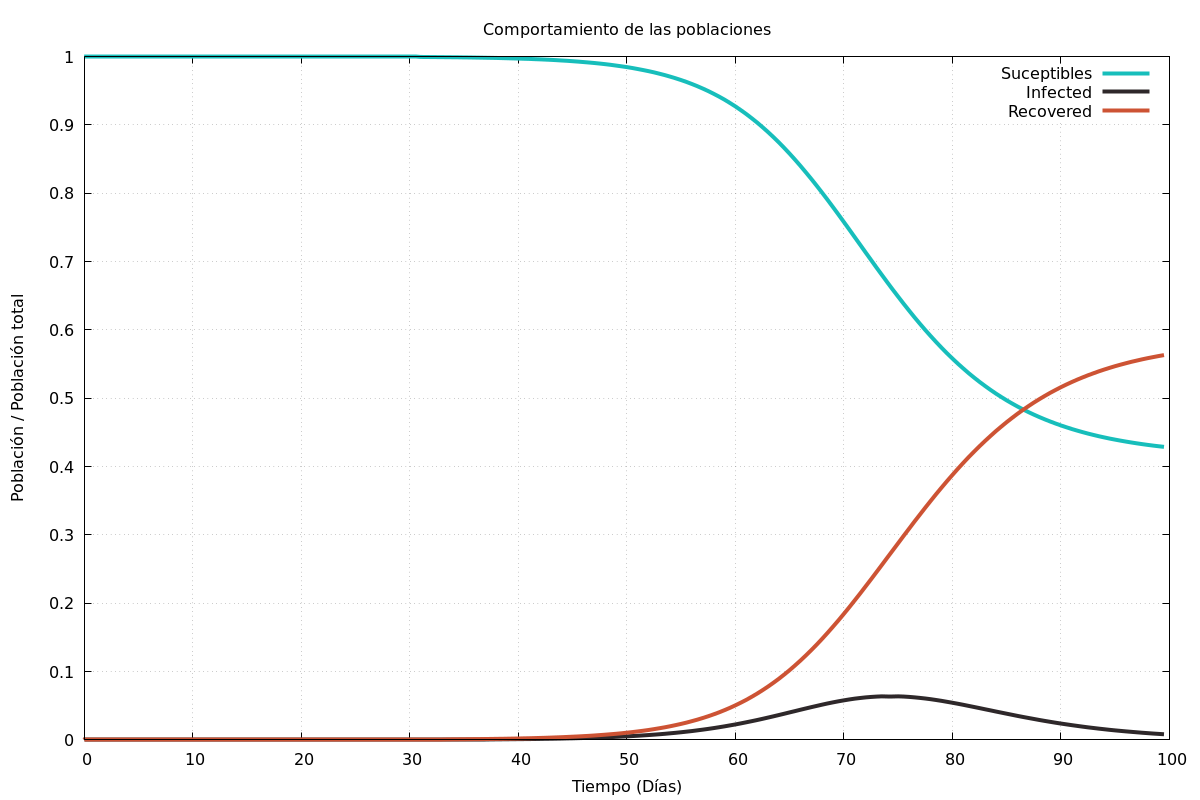
\includegraphics[width=0.5\textwidth]{SIR/graph-1-SIR}
	\caption{Simulación para $b=0.5$ y $k=1/3$}
	\label{simulacion1}
\end{figure}
\begin{figure}[H]
	\centering
	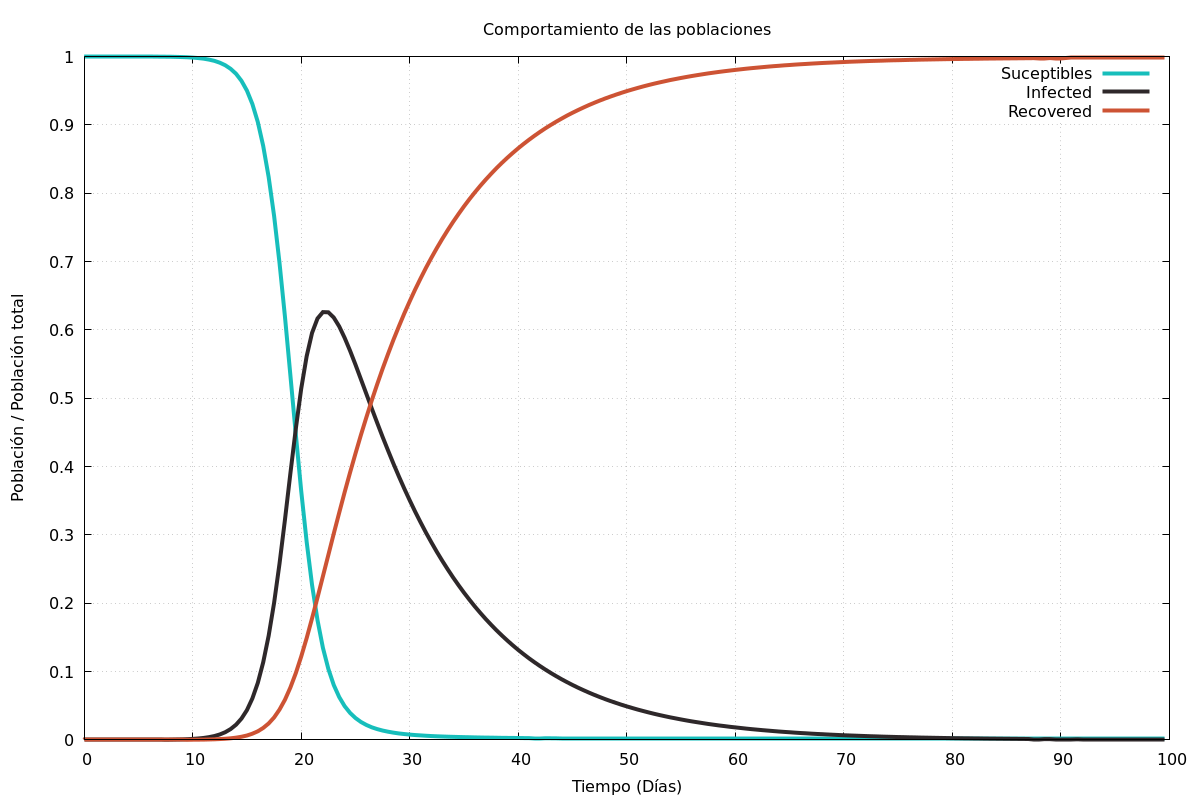
\includegraphics[width=0.5\textwidth]{SIR/graph-2-SIR}
	\caption{Simulación para $b=0.8$ y $k=0.1$}
	\label{simulacion2}
\end{figure}
\begin{figure}[H]
	\centering
	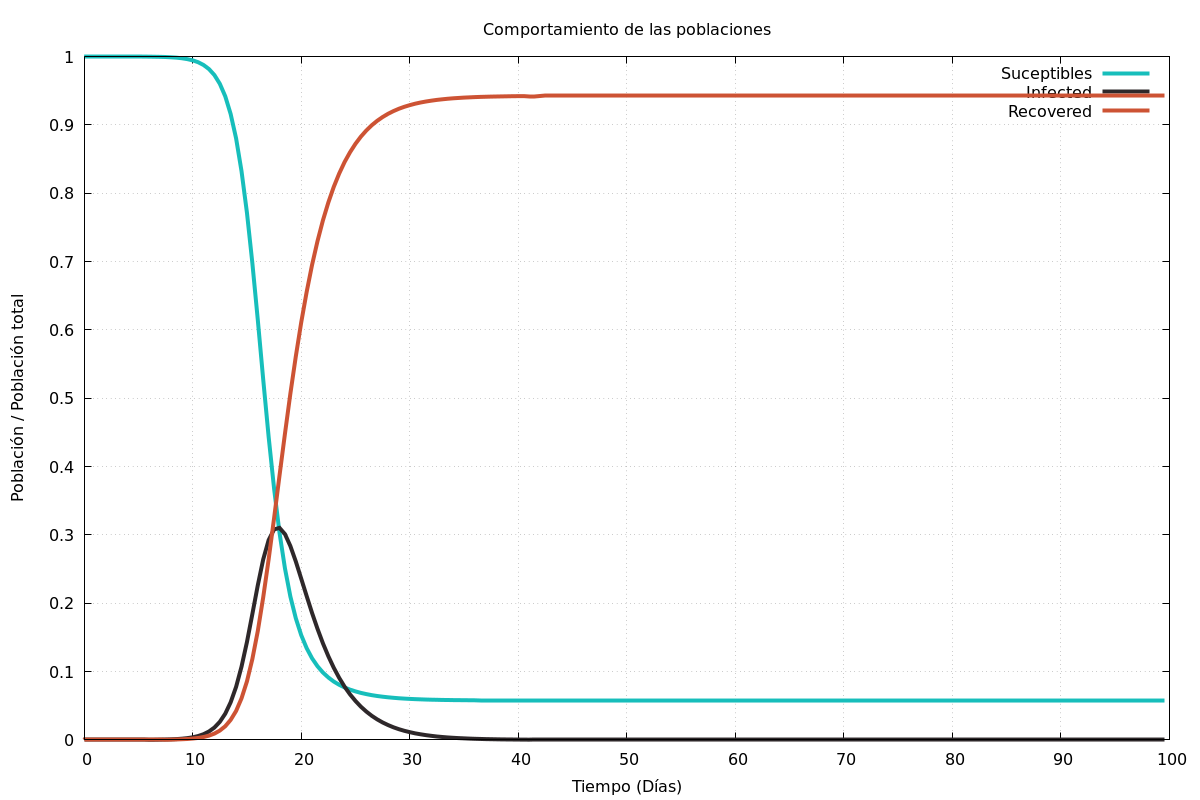
\includegraphics[width=0.5\textwidth]{SIR/graph-3-SIR}
	\caption{Simulación para $b=1.2$ y $k=0.4$}
	\label{simulacion3}
\end{figure}
\begin{figure}[H]
	\centering
	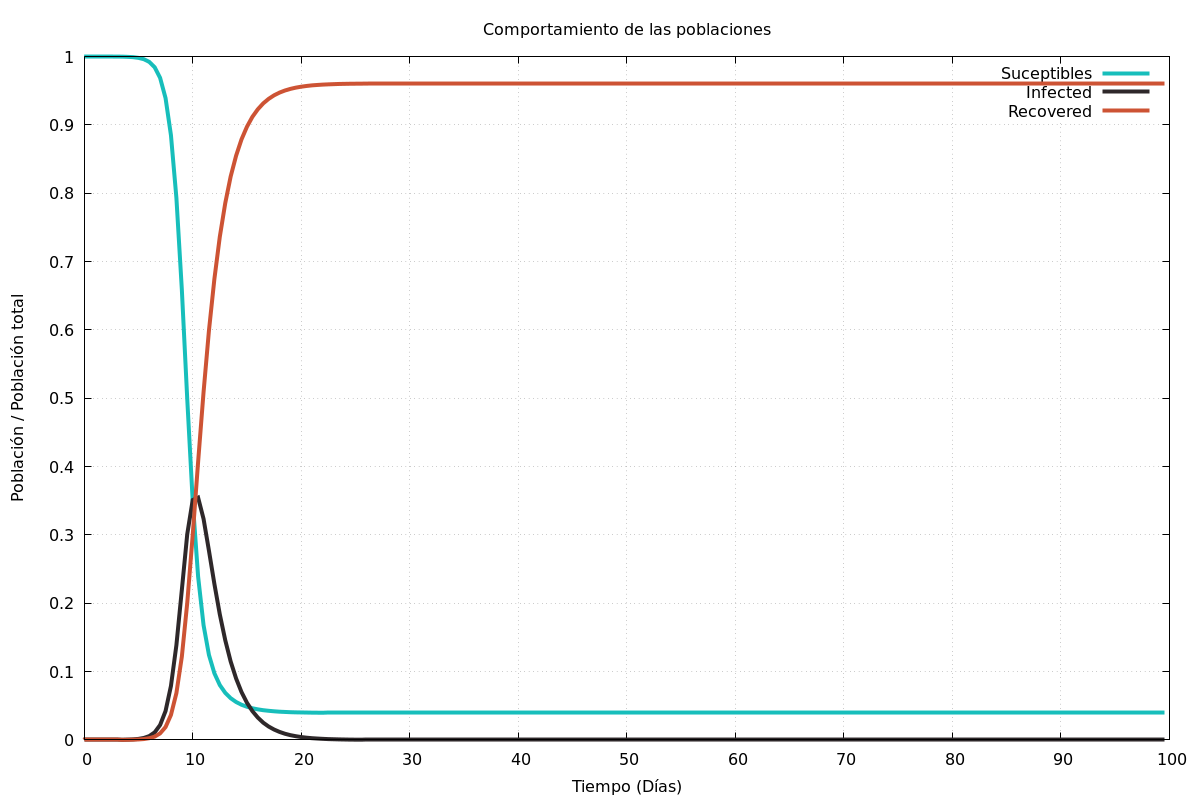
\includegraphics[width=0.5\textwidth]{SIR/graph-4-SIR}
	\caption{Simulación para $b=2$ y $k=0.6$}
	\label{simulacion4}
\end{figure}


La idea ha ido más allá, y con la intención de explorar más el modelo bajo diferentes parámetros, se ha realizado
una representación 3D en una grafica de contorno, en la que se puede observar el 
comportamiento de la población en función de los parámetros.
%%IMAGEN DE GRAFICA DE CONTORNO

Esto obliga realizar las graficas para un momento determinado, es decir el tiempo está fijo. Más sin embargo
para observar el comportamiento de la población en función tanto de los parámetros como del tiempo, se 
realiza una animación tipo \textit{gif}, en la que se puede observar el comportamiento a través del tiempo. 
El \textit{gif} se puede observar en la siguiente dirección \href{https://github.com/niaggar/propagacion-de-enfermedades-project}{Animación-3D} el cual se encuentra tambien dentro del repositorio \cite{GitHub}.

Dentro del proyecto tambien se ha diseñado un codigo que genera de manera automática, reportes en \texttt{LaTeX}, en los que
de manera sencilla, se presenta un informe con todos los resultados arrojados por el programa como el tipo
de modelo utilizado, valores iniciales, y parámetros correspondientes, tiempo de ejecución del programa, y el tamaño de paso utilizado, además de la simulación realizada. 
Tambien se incluye información importante como el  máximo de infectados según el modelo, este pico se calcula con otra 
función tambien dentro del programa. En el caso de los 4 parámetros escogidos en particular [\ref{parametros}],
se tienen los siguientes picos para la población infectada. \\
%%Tabla que contiene los datos de los picos de la población infectada
\begin{table}[H]
	\centering
	\begin{tabular}{|c|c|r|r|l}
	\cline{1-4}
	b   & k   & \multicolumn{1}{c|}{Pico de infectados} & \multicolumn{1}{c|}{día} &  \\ \cline{1-4}
	0.5 & 1/3 & 540,260                                 & 75                       &  \\ \cline{1-4}
	0.8 & 0.1 & 4,944,894                               & 22                       &  \\ \cline{1-4}
	1.2 & 0.4 & 2,450,935                               & 18                       &  \\ \cline{1-4}
	2   & 0.6 & 2,800,676                               & 11                       &  \\ \cline{1-4}
	\end{tabular}
\end{table}


Ha sido de interés explorar otras condiciones iniciales, y en especial nos preguntamos, que sucede si la población de infectados
inicial es 0, claramente se habría de esperar que no se produzca ninguna epidemia, tal como se presenta a continuación;
\begin{figure}[H]
	\centering
	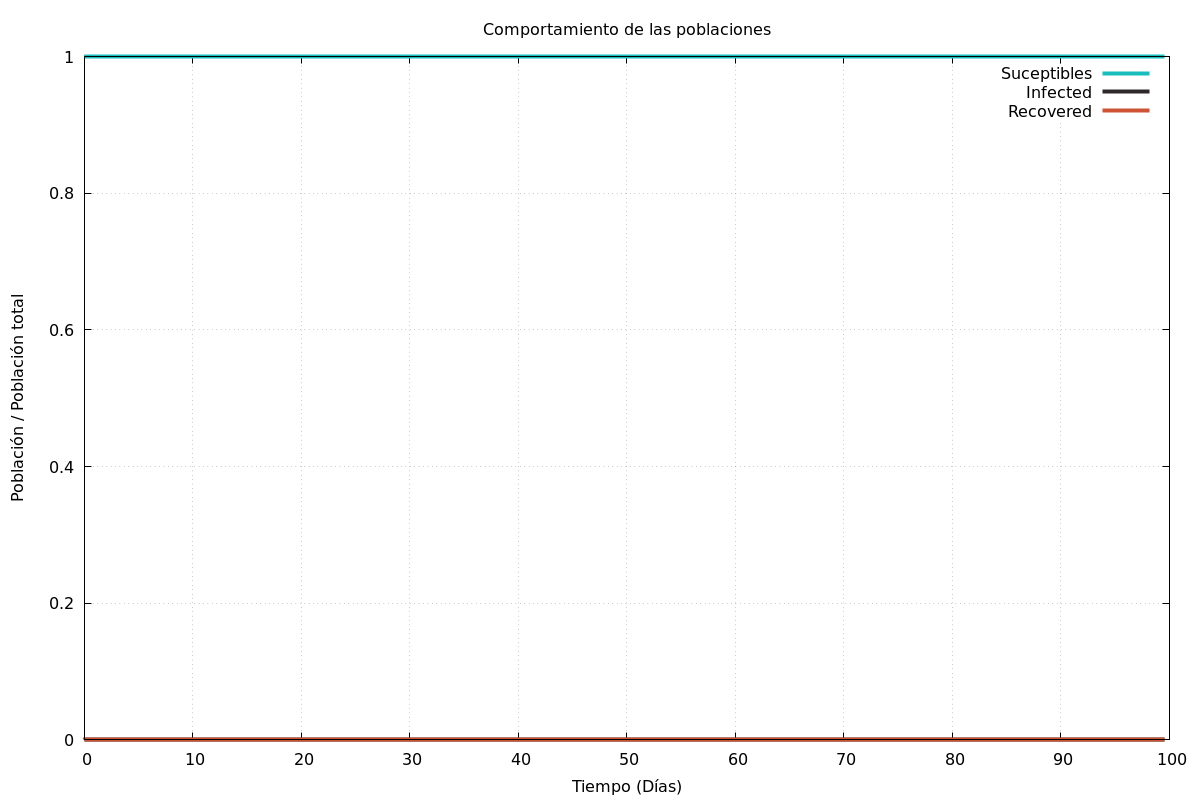
\includegraphics[width=0.5\textwidth]{SIR/graph-i0-SIR}
	\caption{Simulación para $b=0.5$ y $k=1/3$ con $i_0=0$}
	\label{simulacion5}
\end{figure}
	
Por otra parte se ha graficado el diagrama de fases, para cada conjunto de poblaciones, en el que se puede observar 
la variación de la población respecto al tiempo es decir la derivada de la población, contra la población. A continuación se presentan los diagramas de fases para
los parametros escogidos en \ref{parametros}.
\begin{figure}[H]
	\centering
	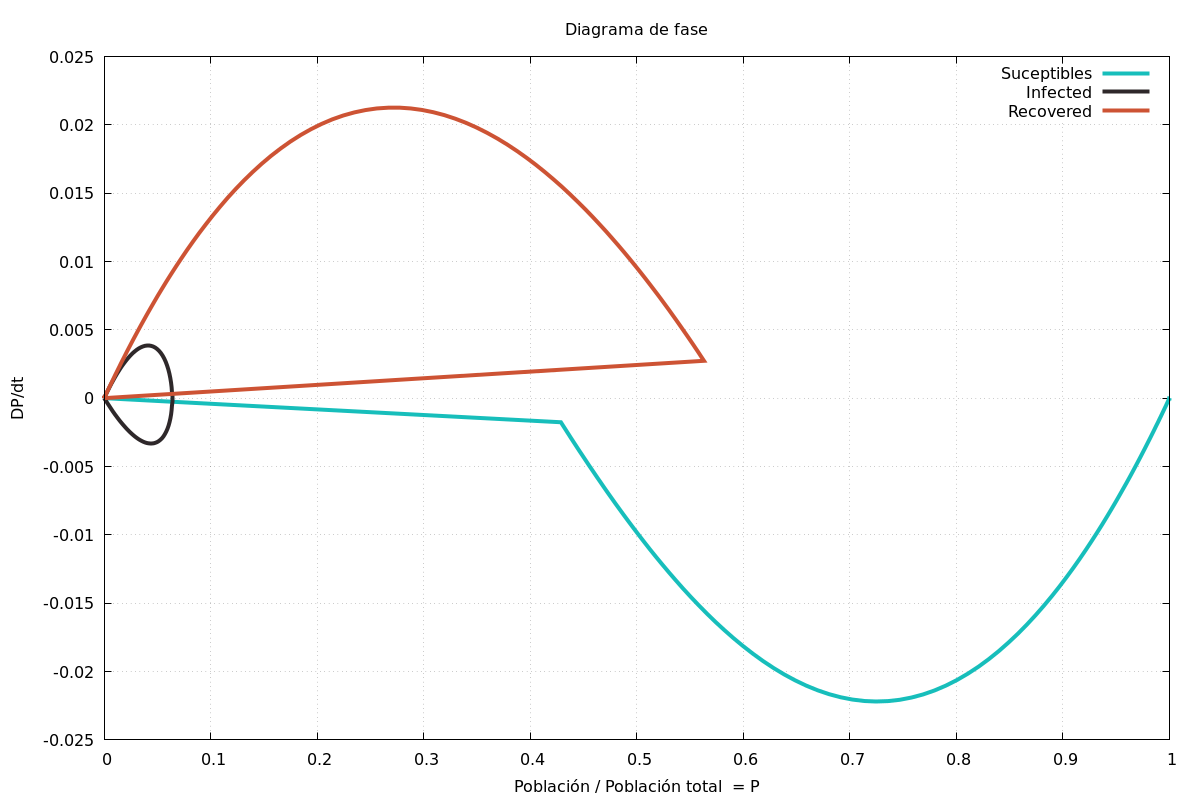
\includegraphics[width=0.5\textwidth]{SIR/phase-1-SIR}
	\caption{Diagrama de fases para $b=0.5$ y $k=1/3$}
	\label{diagrama-fases}
\end{figure}
\begin{figure}[H]
	\centering
	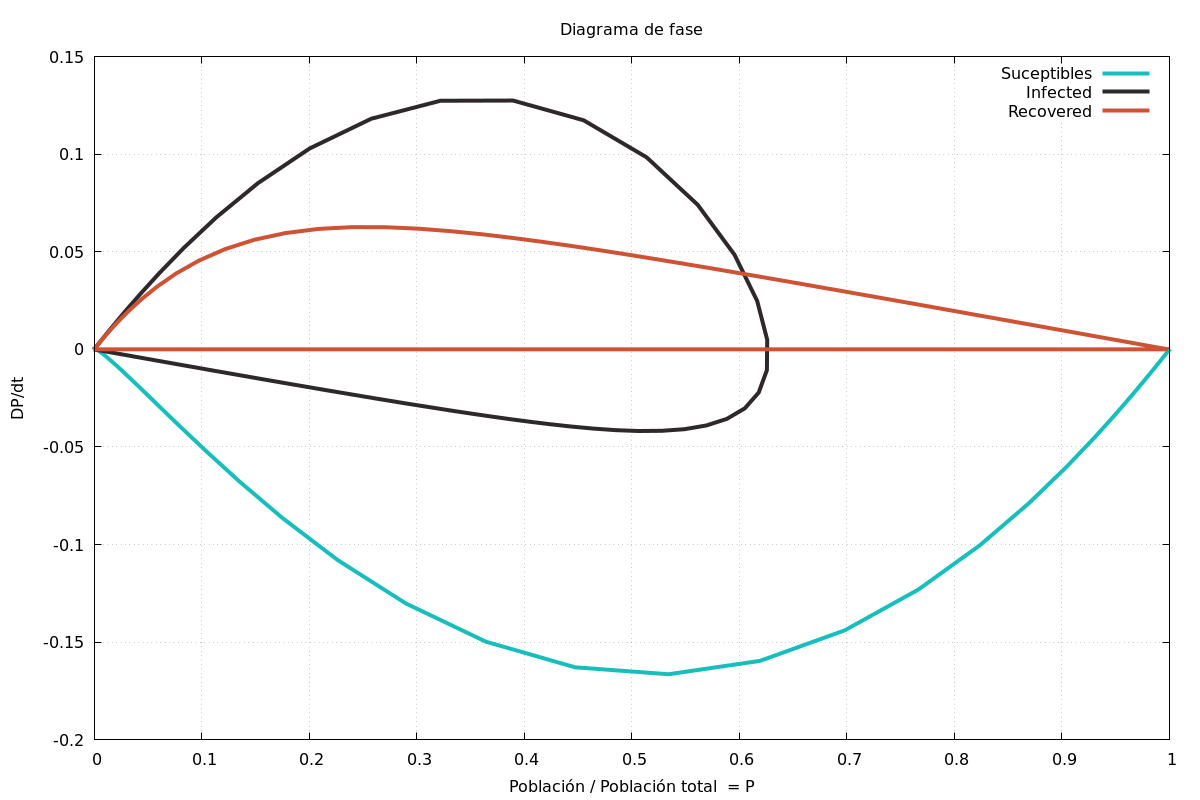
\includegraphics[width=0.5\textwidth]{SIR/phase-2-SIR}
	\caption{Diagrama de fases para $b=0.8$ y $k=0.1$}
	\label{diagrama-fases}
\end{figure}\begin{figure}[H]
	\centering
	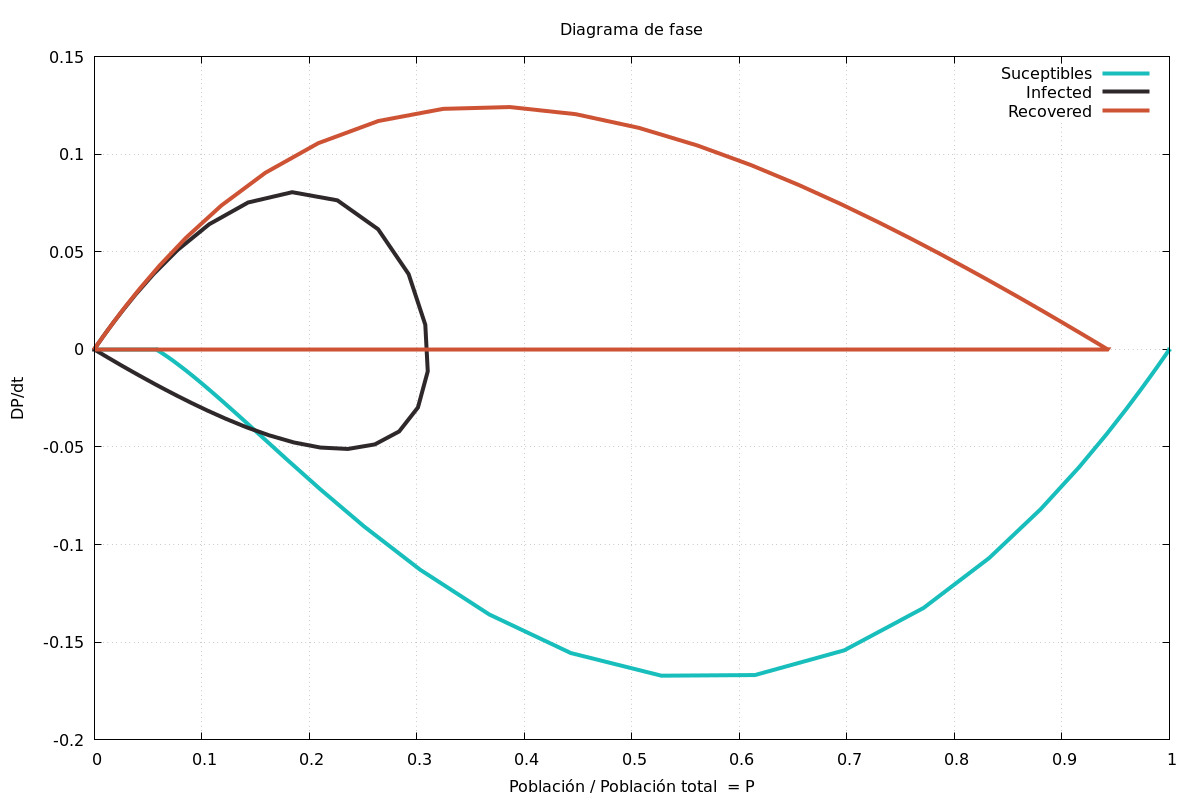
\includegraphics[width=0.5\textwidth]{SIR/phase-3-SIR}
	\caption{Diagrama de fases para $b=1.2$ y $k=0.4$}
	\label{diagrama-fases}
\end{figure}\begin{figure}[H]
	\centering
	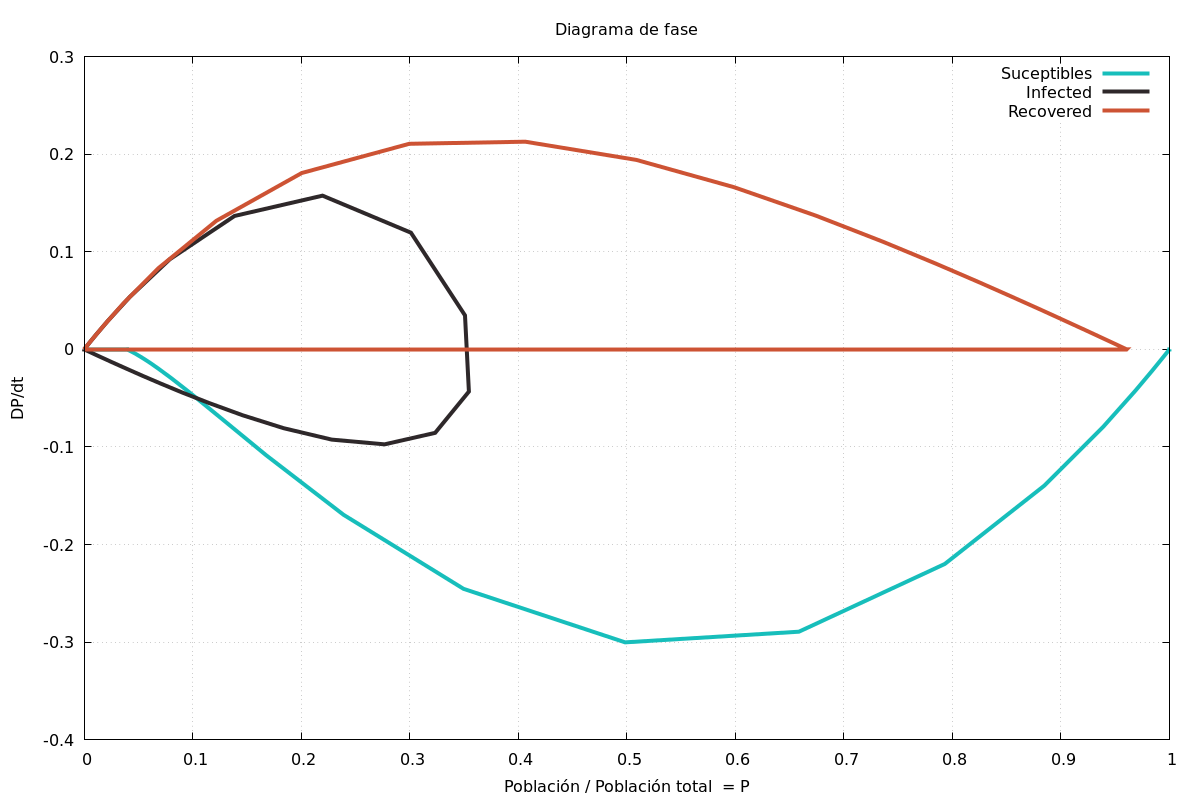
\includegraphics[width=0.5\textwidth]{SIR/phase-4-SIR}
	\caption{Diagrama de fases para $b=2$ y $k=0.6$}
	\label{diagrama-fases}
\end{figure}
	
Por ultimo, se ha creado una simulación tipo \textit{gif}, en el que se aprecian 4 panales, el de la 
esquina superior izquierda contiene el diagrama de fase, y los otros tres paneles 
contienen la población en función del tiempo para cada una de las poblaciones involucradas, 
el gif se puede observar en la siguiente dirección \href{https://github.com/niaggar/propagacion-de-enfermedades-project}{gif-modelo SIR} 
el cual se encuentra tambien dentro del repositorio \cite{GitHub}.

\section{Acercamiento a otros modelos}
%IMPLEMENTACION DEL CODIGO A OTROS MODELOS, SIRS Y SRIS CON VACUNACION
En la sección \ref{Modelos}, se habla acerca de otros modelos de compartimiento, que tienen en cuenta más factores,
mejorando las hipótesis planteadas en el modelo \textit{SIR}, lo que permite
tener modelos más precisos, como es el caso del modelo \textit{SIRS}, e incluso poder añadir
un control de vacunación. A continuación se hablara brevemente acerca de estos dos modelos en concreto,
y el cómo implementar la simulación sobre los mismos con el desarrollo computacional realizado.

\subsection{Modelo SIRS}\label{Modelo SIRS}
El modelo SIR es optimo para describir epidemias en periodos de tiempo no muy amplios
en los que podemos prescindir de los nacimientos y las muertes por causas naturales, superar esta limitación,
permitiría un análisis dinámico en periodos de tiempo más largos. 
Para modelizar este caso, es necesario considerar las muertes por causas externas a la epidemia,
la tasa de natalidad, y si es el caso incluir la tasa de recuperados que regresan a la población infectada (este ultimo depende 
de si la enfermedad provoca o no inmunidad a los individuos que ya fueron infectados). Para realizarlo de manera
más sencilla, se supone que tanto la tasa de natalidad como la mortandad 
siguen un comportamiento malthusiano, y además la población total se mantiene constante, esto se consigue equiparando la
tasa de recién nacidos con las muertes.\\ 

Esta consideración sutil, denomina a este nuevo modelo como \textit{modelo SIR con dinámica vital}\cite{SIRS-VAC}, aunque 
hay que destacar que esta modificación sigue siendo muy modesta, si se busca mejorar mucho más el modelo, 
habría que considerar que la población total $N$ en realidad no es constante, y esto implicaría añadir una nueva
ecuación para $N'$.

El modelo completo se vería en una modificación del sistema \ref{SIR}, de la siguiente forma;

\begin{equation*}
    \begin{split}
      \frac{ds}{dt} = -bs(t)i(t) - \mu s(t) + B,\\
      \frac{di}{dt} = bs(t)i(t)-ki(t)-\mu i(t),\\
      \frac{dr}{dt} = -ki(t) - \mu r(t)\\
    \end{split}
\end{equation*}

Donde se han introducido dos nuevos parámetros, $\mu > 0$ como la tasa de mortalidad por casas naturales 
(este se debe restar a todas las poblaciones), y $B$ que representa la tasa de nacimientos, recién nacidos que se suman
a la población de susceptibles.\\ 

Pero por simplicidad hemos dicho que se mantendrá la suposición \ref{suposicion}, es decir la población
total será constante, por lo que necesariamente $B = \mu N$, y dado que las variables están normalizadas
$N=1$. Haciendo esta consideración, solo añadimos un nuevo parámetro, 
y se obtiene un modelo más sencilla, aunque mejor que el modelo \textit{SIR}, del siguiente modo;

\begin{equation}\label{SIRS}
  \begin{split}
    \frac{ds}{dt} = -bs(t)i(t) + \mu (1 - s(t)) ,\\
    \frac{di}{dt} = bs(t)i(t)-ki(t)-\mu i(t),\\
    \frac{dr}{dt} = -ki(t) - \mu r(t)\\
  \end{split}
\end{equation}

Estas nuevas ecuaciones se han añadido como un nuevo modelo dentro del codigo, y bajo las mismas condiciones iniciales
consideradas en este trabajo, y bajo ahora estos dos conjuntos nuevos de parámetros, en los que $\mu$ es constante;
\begin{equation}\label{parametrosSIRS}
	\begin{split}
		b = 0.8, \quad y \quad k = 0.1\\
		b = 0.5, \quad  y \quad k = 0.2\\
		\mu = 0.06\\
	\end{split}
\end{equation}
Se ha realizado la simulación correspondiente, que se puede observara continuación;
\begin{figure}[H]
	\centering
	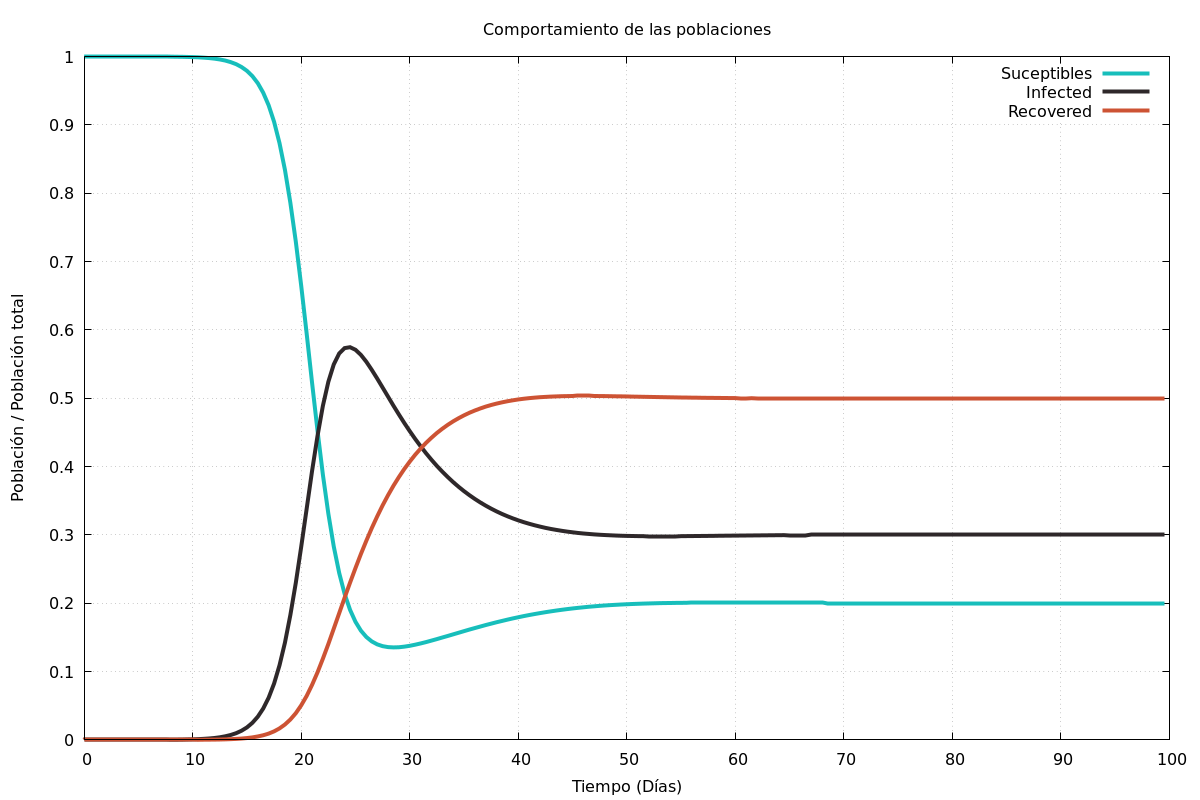
\includegraphics[width=0.5\textwidth]{SIRS/graph-1-SIRS}
	\caption{Simulación del modelo SIRS, con $\mu = 0.06$ y $b = 0.8, k = 0.1$}
	\label{fig:SIRS}
  \end{figure}
\begin{figure}[H]
  \centering
  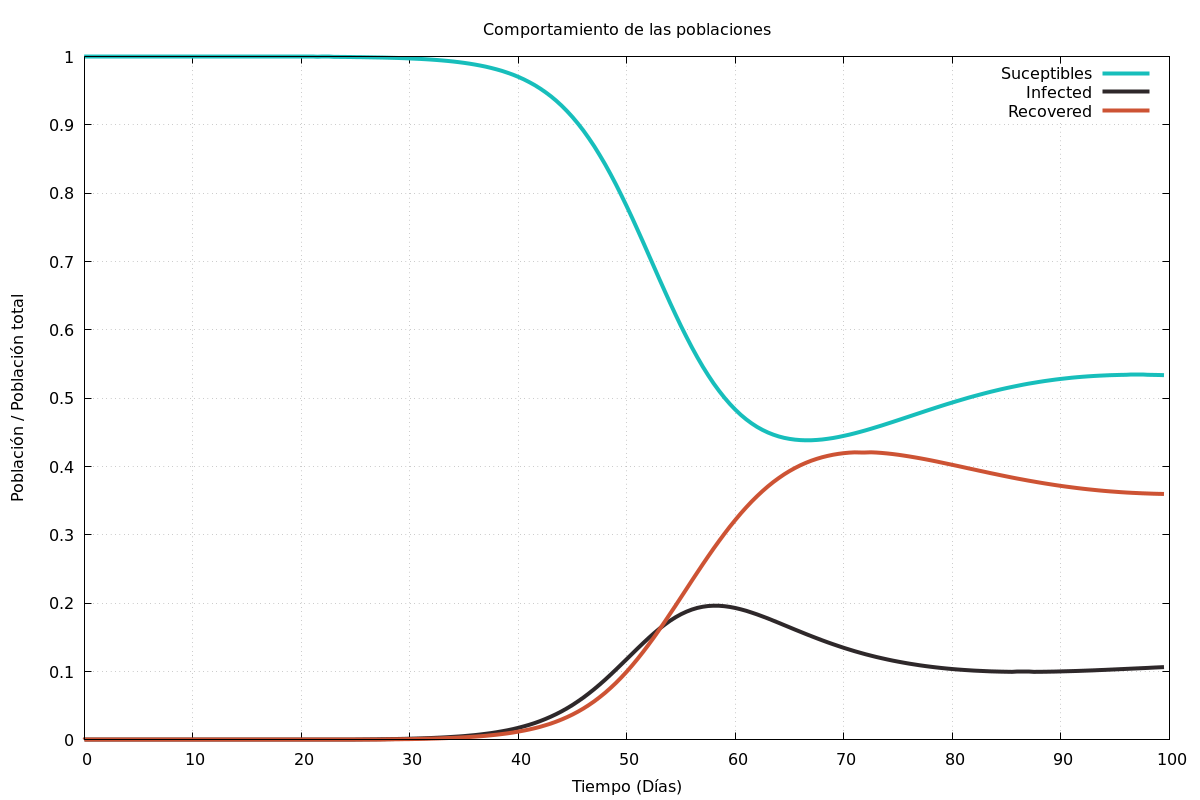
\includegraphics[width=0.5\textwidth]{SIRS/graph-2-SIRS}
  \caption{Simulación del modelo SIRS, con $\mu = 0.06$ y $b = 0.5, k = 0.2$}
  \label{fig:SIRS}
\end{figure}

%%INSERTAR GRAFICAS DEL MODELO SIRS

\subsection{Modelo SIRS con vacunación}
La importancia de estos modelos surge cuando es posible modelar el papel que tiene la vacunación, y existen diversos modelos
que consiguen esto. En este caso se plantea seguir con una extensión del modelo \textit{SIRS} \ref{Modelo SIRS},
para ello se introducen dos nuevos parámetros, $\gamma_1, \gamma_2 \in (0,1)$, que representan la tasa de recién nacidos
y de individuos susceptibles que son vacunados, respectivamente.\\ 

El sistema de ecuaciones diferenciales que define el modelo \textit{SIR} incluyendo la dinámica vital y
la vacunación \cite{SIRS-VAC} está dado por;

\begin{equation}\label{SIRS-VAC}
  \begin{split}
    \frac{ds}{dt} = -bs(t)i(t) + \mu (1 - s(t) -\gamma_1) - \gamma_2 s(t),\\
    \frac{di}{dt} = bs(t)i(t)-ki(t)-\mu i(t),\\
    \frac{dr}{dt} = -ki(t) + \mu (\gamma_1 - r(t)) + \gamma_2 s(t) \\
  \end{split}
\end{equation}

De nuevo estas nuevas ecuaciones se han añadido como un nuevo modelo dentro del codigo, y bajo las mismas condiciones iniciales,
y manteniendo los parámetros \ref{parametrosSIRS} usados en el modelo \ref{Modelo SIRS}, pero añadiendo a $\gamma_1$ y $\gamma_2$ del siguiente modo;
\begin{equation}
	\begin{split}
		\gamma_1 = 0.05, \quad y \quad \gamma_2 = 0.04\\
	\end{split}
\end{equation}

%%INSERTAR GRAFICAS DEL MODELO SIRS-VAC
A continuación se muestra las graficas, que se han obtenido con el modelo \textit{SIRS-VAC}, con los parámetros 
y condiciones iniciales ya establecidas. 
\begin{figure}[H]
	\centering
	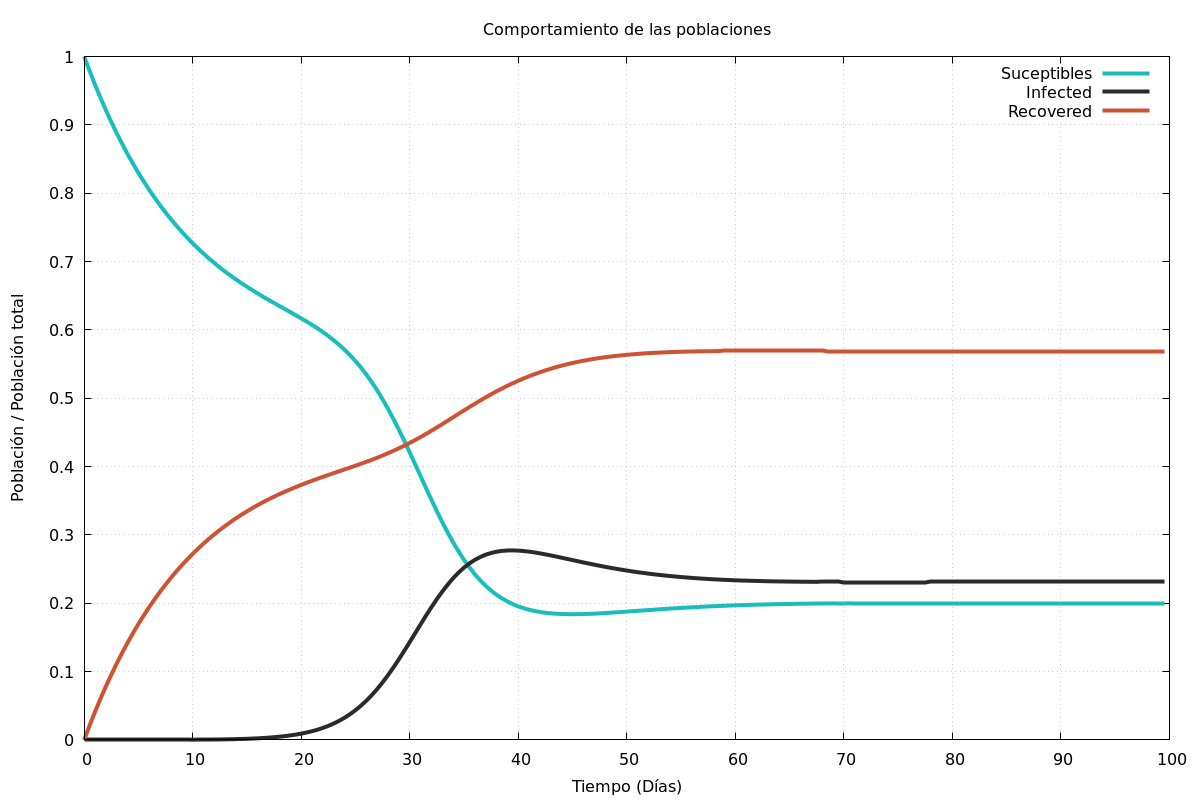
\includegraphics[width=0.5\textwidth]{SIRS/graph-1-SIRSV}
	\caption{Simulación del modelo SIRS-VAC, con $\mu = 0.06, \gamma_1 = 0.05, \gamma_2 = 0.04$ y $b = 0.8, k = 0.1$}
	\label{fig:SIRS-VAC}
\end{figure}
\begin{figure}[H]
	\centering
	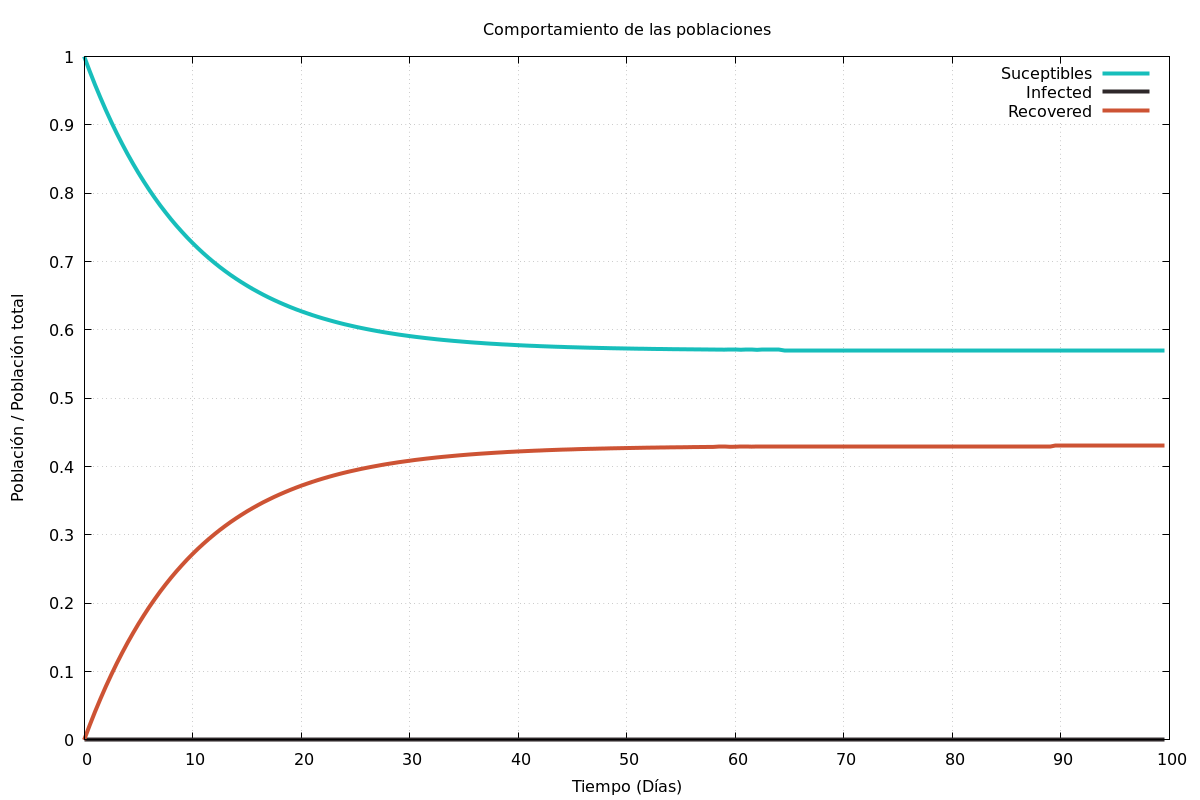
\includegraphics[width=0.5\textwidth]{SIRS/graph-2-SIRSV}
	\caption{Simulación del modelo SIRS-VAC, con $\mu = 0.06, \gamma_1 = 0.05, \gamma_2 = 0.04$ y $b = 0.5, k = 0.2$}
	\label{fig:SIRS-VAC}
\end{figure}


%%%%%%%%%%%%%%%%%%%%%%%%%%%%%%%%%%%%%%%%%
%%%%%%%%%%% SECCIONES FINALES %%%%%%%%%%% 
%%%%%%%%%%%%%%%%%%%%%%%%%%%%%%%%%%%%%%%%%
\section{Resultados}
%%SOLUCION A LAS PREGUNTAS PLANTEADAS 
Tras todo el trabajo presentado, es importante rescatar los resultados obtenidos, ya que se presenta un codigo que permite,
de manera sencilla para el usuario obtener un análisis de los modelos \textit{SIR} donde se pueda introducir de manera 
particular los parámetros y valores iniciales a usar, e incluso implementar algún otro modelo que desee
en nuestro caso únicamente se han implementado los modelos \textit{SIRS} y \textit{SIRS} con vacunación, pero se puede extender el codigo
a cualquier otro modelo. Tambien es de resaltar las animaciones tipo \textit{GIF} realizadas, y en especial la animación de la evolución
temporal, de los poblaciones en función de los parámetros, que en retrospectiva es una forma de visualizar un función de 3 variables, 
una temporal, y dos más que son los parámetros $b$ y $k$, una tarea que no fue sencilla de realizar, pero que se ha conseguido con éxito,
y que resulta muy interesante para el usuario, ya que permite ver de manera gráfica como evoluciona el modelo en función de los parámetros\\
%%%%%%%%%%%%%%%%%%%%%%%%%%%
%%%%%%%%%%%%%%%%%%%%%%%%%%%%%%%%%%%%%
%%%%%%%%%%%% CONCLUSIONES %%%%%%%%%%%
%%%%%%%%%%%%%%%%%%%%%%%%%%%%%%%%%%%%%
\section{Conclusiones}
A manera de discusión sobre los resultados obtenidos en la sección \ref{simulaciones}, es claro observar que en las graficas 
de evolución de las poblaciones bajo diferentes parámetros, presenta en general una misma tendencia de comportamiento, solo
que alcanzando diferentes picos, y con diferentes tiempos de evolución, pero en general se puede observar que la población, se comporta de manera similar.
El pico más bajo se alcanza en la grafica \ref{simulacion1}, en este caso en particular, se puede observar que las poblaciones
de susceptibles y recuperados, evolucionan de forma más lenta, y sin alcanzar los extremos, es decir si se observa las otras graficas 
se puede observar que las poblaciones de susceptibles y recuperados, alcanzan picos mucho más altos, llegando los recuperados al $100\%$ de la población, y en menor tiempo, pero en este caso
la población de recuperados y susceptibles parecen quedarse en un punto intermedio, y de igual manera la población de infectados,
parece no desaparecer, manteniendo la epidemia.\\

Por otra parte los demás modelos \textit{SIRS} y \textit{SIRS} con vacunación, presentan curvas más "suaves", y trayendo a colación



\ifCLASSOPTIONcaptionsoff
	\newpage
\fi

%%%%%%%%%%%%%%%%%%%%%%%%%%
%%%%%% BIBLIOGRAFIA %%%%%%
%%%%%%%%%%%%%%%%%%%%%%%%%%
\begin{thebibliography}{1}

	\bibitem{Ross}
	Ross R.. The prevention of malaria (2nd edition, with Addendum). John
	Murray, London. 1911.
	\bibitem{Kermack}
	Kermack, W. O. and McKendrick, A. G. . A Contribution to the
	Mathematical Theory of Epidemics
	Royal Society of London Proceedings Series A. 1927;115:700–721.
	\bibitem{compartimientos}
	J. Aracil. Introducción a la dinámica de sistemas. Alianza Universidad Textos.
	Mexico. 1986.Biosciences Subseries. Springer 2008
	\bibitem{SIDA}
	Driessche P. Wu J. (Eds.). Mathematical Epidemiology (Lecture Notes in
	Mathematics / Mathematical
	Biosciences Subseries). Springer 2008.
	\bibitem{Rubeola}
	Brauer, F. and Castillo-Chávez, C. . Mathematical Models in Population
	Biology and Epidemiology.
	Springer, New York 2012.
	\bibitem{Dengue}
	Esteva L. Vargas C.. Analysis of a dengue disease transmission model.
	Mathemtical Biosciences.
	1998;150:131–151.
	\bibitem{Influenza}
	Pava E. De. Modelado Matemático de la transmisión de gripe AH1N1.
	Matemáticas Enseanza
	Universitaria.. 2010;XVIII:1–10.
	\bibitem{Vacunacion}
	Hernández, M. E. (2021). Vacunación óptima para un modelo SIRS. Revista
	De Educación Matemática, 29(2).
	Recuperado a partir de
	\url{https://revistas.unc.edu.ar/index.php/REM/article/view/10055}.
	\bibitem{Anderson}
	Anderson R. M.. Population Dynamics of infectious diseases: Theory and
	Application. Chapman
	Hall, London 1982.
	\bibitem{Sulucion_analitica}
	Alexsandro M. Carvalho and Sebastián Gon¸calves. An Algebraic Solution
	for the Kermack-McKendrick Model, sep-2016.
	arXiv e-prints, 1609.09313, physics.soc-ph.
	\bibitem{GitHub}
	Andres Valencia and Nicolas Aguilera, Project: Propagación de
	enfermedades in C++
	Fisica Computacional, Enero-2023, Cali Valle.
	\url{https://github.com/niaggar/propagacion-de-enfermedades-project}.
	\bibitem{Runge-kutta}
	J. Arrieta, R. Ferreira, R. Pardo y A. Rodríguez-Bernal. Análisis Numérico
	de Ecuaciones Diferenciales Ordinarias.
	Paraninfo, Madrid, 2020. ISBN 9788428344418, ISBN 8428344418.
	\bibitem{Modelos de propagacion}
	Fred Brauer, Modelos de la propagación de enfermedades infecciosas,
	Universidad Autónoma de Occidente, 2015. ISBN	958871365X, 9789588713656.
  \bibitem{SIRS-VAC}
  García Piñera Andrea, Modelos de ecuaciones diferenciales para la propagación de enfermedades.
  2014, \url{http://hdl.handle.net/10902/7125}
\end{thebibliography}
%%%%%%%%%%%%%%%%%%%%%%%%%%

\end{document}
%%%%%%%%%%%%%%%%%%%%%%%%%%%%%%%%
%%%%%% FIN DEL DOCUMENTO %%%%%%%
%%%%%%%%%%%%%%%%%%%%%%%%%%%%%%%%